\documentclass{standalone}
\usepackage{tikz}
\usepackage{ctex,siunitx}
\setCJKmainfont{Noto Serif CJK SC}
\usepackage{tkz-euclide}
\usepackage{amsmath}
\usetikzlibrary{patterns, calc}
\usetikzlibrary {decorations.pathmorphing, decorations.pathreplacing, decorations.shapes,}

\begin{document}
\small
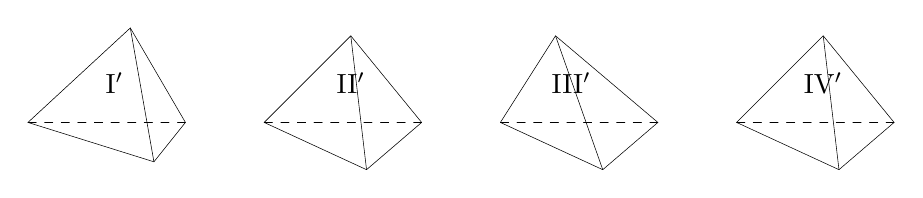
\begin{tikzpicture}[>=stealth,scale=1]
  \tkzSetUpPoint[fill=black]
  % \useasboundingbox(-1,-0.75)rectangle(3.7,1.4);
\begin{scope}
	\tkzDefPoints{0/0/A, 2/0/B, 1.3/1.2/C, 1.6/-.5/D}
	\tkzDrawPolygon(A,D,B,C)
	\tkzDrawSegments[dashed](A,B)
	\tkzDrawSegments(C,D)
\node at (1.1,.5){I$'$};
\end{scope}
\begin{scope}[xshift=3cm]
	\tkzDefPoints{0/0/A, 2/0/B, 1.1/1.1/C, 1.3/-.6/D}
	\tkzDrawPolygon(A,D,B,C)
	\tkzDrawSegments[dashed](A,B)
	\tkzDrawSegments(C,D)
	\node at (1.1,.5){II$'$};
\end{scope}
\begin{scope}[xshift=6cm]
	\tkzDefPoints{0/0/A, 2/0/B, 0.7/1.1/C, 1.3/-.6/D}
	\tkzDrawPolygon(A,D,B,C)
	\tkzDrawSegments[dashed](A,B)
	\tkzDrawSegments(C,D)
	\node at (.9,.5){III$'$};
\end{scope}
\begin{scope}[xshift=9cm]
	\tkzDefPoints{0/0/A, 2/0/B, 1.1/1.1/C, 1.3/-.6/D}
	\tkzDrawPolygon(A,D,B,C)
	\tkzDrawSegments[dashed](A,B)
	\tkzDrawSegments(C,D)
	\node at (1.1,.5){IV$'$};
\end{scope}
\end{tikzpicture}
\end{document}